% 论文 1037 中文译稿：与 main.tex（v25，2026-11-09）逐段、逐句对应；图片沿用英文原图，图注与表格已译。
% 编译：tectonic -X compile main_zh.tex（XeLaTeX；中文字体为 Fandol，由 TeX 发行版提供）。
% 仅供阅读核对；投稿以英文 main.tex 为准。
\documentclass{vgtc_zh}
\usepackage[T1]{fontenc}
\usepackage{mathptmx}
\usepackage{xeCJK}
\setCJKmainfont{FandolSong-Regular.otf}[BoldFont=FandolHei-Regular.otf,ItalicFont=FandolKai-Regular.otf]
\setCJKsansfont{FandolHei-Regular.otf}
\xeCJKsetup{CJKecglue={ }}
% xeCJK loads fontspec, which would replace mathptmx's Times text with Latin Modern; use the TeX Gyre clones instead.
\setmainfont{texgyretermes}[Extension=.otf,UprightFont=*-regular,BoldFont=*-bold,ItalicFont=*-italic,BoldItalicFont=*-bolditalic]
\setsansfont{texgyreheros}[Extension=.otf,UprightFont=*-regular,BoldFont=*-bold,ItalicFont=*-italic,BoldItalicFont=*-bolditalic]
\usepackage{cite}
\usepackage{amsmath,amssymb,amsthm}
\usepackage{placeins}
\usepackage{booktabs,multirow,colortbl}
\makeatletter
\setlength{\@dblfptop}{0pt}
\setlength{\@dblfpsep}{12pt}
\setlength{\@dblfpbot}{0pt plus 1fil}
\makeatother
\setcounter{dbltopnumber}{2}
\setcounter{secnumdepth}{3}
\newtheorem{theorem}{定理}
\newtheorem{lemma}{引理}
\newtheorem{proposition}{命题}
\renewcommand{\proofname}{证明}
\renewcommand{\abstractname}{摘要}
\AtBeginDocument{\renewcommand{\figurename}{图}\renewcommand{\tablename}{表}}
\newcommand{\dtop}{d_{\mathrm{top}}}
\newcommand{\lca}{\operatorname{lca}}
\newcommand{\nroe}{\mathrm{NROE}}
\onlineid{1037}
\vgtccategory{Research}
\vgtcinsertpkg

\title{AnchorMTM：带位置下界的空间锚定合并树地图}

\author{%
Lele~Wang$^{1,2}$\thanks{%
单位：
$^{1}$ 中国科学院计算机网络信息中心先进交互式技术与应用研究室，北京；
$^{2}$ 中国科学院大学，北京；
$^{3}$ 国科大杭州高等研究院，杭州。
邮箱：lelewang@cnic.cn；dongyu@cnic.cn；yxmeng@cnic.cn；
liguan@sccas.cn；wangzhe@sccas.cn；sgh@sccas.cn；
liujun@sccas.cn。
Lele Wang 与 Yu Dong 对本文贡献相同。
Jun Liu 为通讯作者。}%
\quad
Yu~Dong$^{1,*}$%
\quad
Yuxiang~Meng$^{1,2}$%
\quad
Guan~Li$^{1,2}$%
\quad
Zhe~Wang$^{1,2}$%
\quad
Guihua~Shan$^{1,2,3}$%
\quad
Jun~Liu$^{1,2}$\thanks{通讯作者。邮箱：liujun@sccas.cn。}
}

\teaser{
\centering
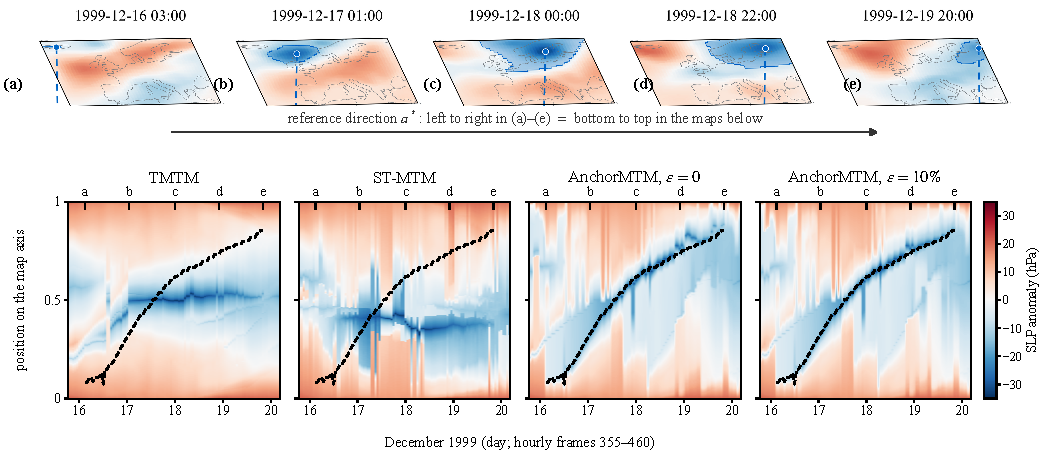
\includegraphics[width=\linewidth]{figures/teaser_storms_compare.pdf}
\par\vskip\abovecaptionskip
\refstepcounter{figure}\label{fig:storms_overview}%
{\captionfonts\leftskip=0pt\rightskip=0pt\parfillskip=0pt plus 1fil\noindent 图~\thefigure：四张合并树地图中的同一个风暴。(a)--(e)~1999 年 12 月 16--19 日北大西洋和欧洲上空的海平面气压距平。标出的低压从大西洋洋面移到斯堪的纳维亚，也就是沿参考方向 $a^*$ 从左向右移动。下方四张地图绘制相同的 106 个逐小时帧；虚线是风暴位置的投影，即轴若表示位置、风暴应当画在的地方。TMTM 和 ST-MTM 把风暴保持在轴的中部附近。AnchorMTM 以精确的树（$\varepsilon=0$；平均偏差为轴长的 1.5\%）和 10\% 的合并误差预算（1.0\%）跟随它。\par}
}

\abstract{合并树地图用一张静态图像概括时变标量场。每个时间步变为其合并树的一维剖面，剖面沿时间堆叠，使嵌套的特征呈现为嵌套的条带。然而，这些地图的纵轴没有空间含义：分析人员能看到特征如何嵌套，却看不出它们在哪里、往哪里移动。我们提出 AnchorMTM，一种纵轴为固定空间方向的合并树地图，每个极值都绘制在其位置的投影附近。在这样的轴上保持树需要付出代价。精确剖面让每棵子树占据一个连续的块，而兄弟子树的投影位置可能相互交错。我们推导出这一冲突所迫使的位移的三个下界，分别对应精确的树、有限宽度的特征和有界的合并层级变化。这些下界只依赖数据，因此在画出任何地图之前就已知道。AnchorMTM 直接从场序列和一个参数计算地图，这个参数是合并误差预算，它限定可以拿多少合并层级的保真度去换取位置。它在 614 个基准帧中的 606 个上达到下界。这些下界还表明，已有合并树地图的排序误差有 31--95\% 并非由树所迫使。在精确保持树的条件下，AnchorMTM 把 TMTM 和 ST-MTM 的平均最坏位移在五个平面序列上降低 73--96\%，在两组体数据上降低 63--67\%，而 ST-MTM 的邻域保持更好。}
\keywords{时变标量场，合并树地图，拓扑保持，空间保真度，下界，约束布局。}
\begin{document}
\firstsection{引言}
\maketitle
\raggedbottom
\setlength{\emergencystretch}{1.5em}
时变标量场记录海平面气压、气溶胶浓度或涡量等量在空间区域上的演变。分析人员借助特征来研究它们，例如低压系统、污染过程或涡旋，并对每个特征提出三个问题：它与其他特征是什么关系，它在哪里，它如何移动。动画让每个时间步保留其空间语境，但难以比较相隔较远的时刻~\cite{Tversky:2002:Animation,Robertson:2008:Animation}。因此，静态总览把一条显示轴分给时间，把空间压缩到另一条轴上，使整个序列放进一张图中~\cite{Bach:2017:STC}。大气科学中的 Hovm\"oller 图是经典例子：它的第二条轴是经度等物理坐标，向东移动的系统表现为一条斜的条纹~\cite{Hovmoller:1949}。为得到这条轴，该图沿其余坐标对场取平均，位于同一经度的特征会混成一个。

合并树地图回答第一个问题，而这正是 Hovm\"oller 图做不到的。合并树记录随阈值升高下水平集分量如何连接：叶子是极值，内部节点是区域合并的层级~\cite{Heine:2016:Survey}。时间合并树地图（TMTM）把每个时间步的树绘制成一维剖面，其极小值是极值、屏障是合并层级，并把剖面堆叠成一张图~\cite{Koepp:2023:TMTM}。时空合并树地图（ST-MTM）还按特征之间的两两距离来排列它们~\cite{STMTM:2026}。第二个问题仍未解决。这些地图的纵轴遵循树和时间连贯性，或遵循相对距离，二者都没有在空间中固定原点或方向。图~\ref{fig:storms_overview} 展示了其后果。一个风暴在三天内横穿北大西洋，两张地图却始终把它画在轴的中部附近；读者看得到风暴如何与相邻低压相连，却看不出它在哪里、向哪边移动。

我们让纵轴具有空间含义。我们在区域中固定一个方向，并给每个极值一个参考位置，即其位置在该方向上的投影；一张表示位置的地图应当把每个极值画在其参考位置上。障碍来自树本身。剖面只有在每棵子树占据一个连续块时才能精确地显示树，但两棵兄弟子树的参考位置可能相互交错（图~\ref{fig:projection_conflict}）。这时，无论用什么算法绘制，都没有精确剖面能把每个特征放在其参考位置上。这一冲突引出三个问题：树迫使多少位移，这些位移源自树的哪里，以及要放弃多少合并层级的保真度才能消除它。没有这些答案，就无法判断一张地图的位置误差来自数据还是来自布局，分析人员也无法判断一条空间轴是否值得其代价。

AnchorMTM 回答这些问题并绘制地图。它以场序列和一个数，即合并误差预算 $\varepsilon$，为输入，直接计算地图；它不是对另一张地图布局的后处理。参考方向由极值的运动估计，或由分析人员选定。仅凭树和参考位置，三个下界就给出精确的树、有限的特征宽度和有界的合并误差所迫使的位移，因此在计算任何布局之前，空间轴的代价就已知道。随后，AnchorMTM 逐帧在符合预算的叶序中选出可达位移最小的一个，在该叶序允许的范围内把极值尽量放在参考位置附近，并填充剖面。当 $\varepsilon=0$ 时，地图精确显示每一棵树；当 $\varepsilon>0$ 时，它把特征移得更靠近参考位置，并报告每一帧实际花掉的合并误差。

本文的贡献如下。
\begin{itemize}
\setlength{\itemsep}{2pt}
\setlength{\parsep}{0pt}
\item 我们提出 AnchorMTM，一种纵轴为固定空间方向的合并树地图。它根据极值位置的投影构建每一帧的叶序和极值位置，使条带的高度读作位置、条带的漂移读作沿该方向的运动，同时剖面保留树的嵌套和合并层级。
\item 我们形式化了保持树与保持位置之间的冲突，并推导出它所迫使的位移的三个下界，分别对应精确的树、有限的特征宽度和有界的合并误差。这些下界不需要布局；它们在树中定位冲突，并能衡量任何合并树地图，包括已有的地图。
\item 我们引入合并误差预算 $\varepsilon$，限定可以拿多少合并层级的保真度去换取位置。一个闭式检验判定一个叶序是否符合预算，并给出它的最优合并屏障，于是一个参数就控制了整个构建，每个渲染帧都按它核验。
\item 在五个平面序列和两组体数据上，下界在 614 个平面帧中的 606 个上达到，已有地图的大部分排序误差被证明是可以避免的，并且在相同的拓扑保证下，AnchorMTM 把特征画得离其位置近得多。
\end{itemize}

\section{相关工作}\label{sec:related}
\subsection{空间数据的时间总览}
动画保留每个时间步的空间语境，静态总览则让观察者直接比较相隔较远的时刻；哪一种更好取决于任务~\cite{Tversky:2002:Animation,Robertson:2008:Animation}。Bach 等人把两者及其相互转换描述为时空立方体的变换~\cite{Bach:2017:STC}。静态总览必须把空间线性化。Hovm\"oller 图保留一个物理坐标并对其余坐标取平均~\cite{Hovmoller:1949}。地理排序、稠密像素显示和空间填充曲线遍历整个区域~\cite{Guo:2006:SpatialOrder,Dafner:2000:CSFC,Rauscher:2025:1DO}，体线和数据驱动曲线把这类遍历扩展到体数据~\cite{Weissenboeck:2019:DVL,Zhou:2021:DSF}。对于运动对象，一维投影以及 MotionRugs、稳定视觉摘要和 MoReVis 等摘要按位置或稳定性对对象排序~\cite{Franke:2021:1DP,Buchmueller:2019:MR,Wulms:2021:SVS,Valdrighi:2024:MRV}。任何线性化都会扭曲部分空间关系~\cite{Nonato:2019:MP,Aupetit:2007:VD}。这些总览保留了空间坐标，却没有特征层级；AnchorMTM 保留合并树，并说明此时空间坐标的代价。

\subsection{时变标量场的拓扑}
合并树和等值线树概括水平集如何连接，基于持续性的简化控制其规模~\cite{Heine:2016:Survey,Edelsbrunner:2002:TPS,Tierny:2018:TTK}。特征通过区域重叠或属性相似性在时间上被追踪~\cite{Silver:1997:Tracking,Saikia:2017:GFT}，并显示为追踪图和嵌套追踪图~\cite{Widanagamaachchi:2012:DTG,Lukasczyk:2017:NTG,Lukasczyk:2020:DNTG}。时变合并树已用 Wasserstein 距离和几何感知交错距离计算与比较~\cite{Oesterling:2017:TVMT,Pont:2022:WMT,Yan:2022:GAMT,Yan:2021:Survey}，这类流程被用于跟踪热带气旋和大气河~\cite{Yan:2024:TROPHY,Lan:2024:AR}。我们所界定的合并误差是一种带标签的交错距离~\cite{Munch:2019:LINF,Gasparovic:2024:IID,Morozov:2013:IDMT}，并与有序合并树之间的距离相关~\cite{Beurskens:2025:OMT}。追踪图显示特征如何出现、分裂和合并，却不显示它们在哪里；合并树地图还显示每个时间步的数值和嵌套，AnchorMTM 再加上它们的位置。

\subsection{一维绘制层级}
拓扑地形把合并树绘制成地形，或绘制成一维剖面，其极小值是极值、屏障是合并层级~\cite{Weber:2007:TL,Oesterling:2013:TLP}；也有保持几何和时间连贯的变体~\cite{Beketayev:2012:GPTL,Herick:2020:TCTL}，等值线树还被绘制在平面上或联合布局中~\cite{Heine:2011:DCT,Lohfink:2020:FCT}。时间树图沿时间布局演化的层级~\cite{Koepp:2019:TT}。TMTM 把相继合并树的剖面对齐成一张静态地图~\cite{Koepp:2023:TMTM}，ST-MTM 加入相对空间距离和时间稳定性~\cite{STMTM:2026}。故事线布局对实体分组面临相关的问题，在交叉和摆动与分组连续性之间权衡~\cite{Tanahashi:2012:Storyline,Liu:2013:SF}。在所有这些布局中，轴上的位置编码的是树的遍历、时间对齐或相对距离。AnchorMTM 让它编码位置。

\subsection{层级与外部顺序}
只要树必须遵从一个外部顺序，就会出现我们研究的冲突。最优叶序为树状图选择与树一致、并让相似叶子相邻的顺序~\cite{BarJoseph:2001:OLO,Eisen:1998:CA}，树重排寻找与树一致且最接近目标顺序的排列~\cite{Bulteau:2022:RT}。空间有序树图和数据--空间网格图在层级或数据布局与地理位置之间权衡~\cite{Wood:2008:SOT,vanBeusekom:2023:DSL}，地理系统发育把叶序与地图位置联系起来~\cite{Klawitter:2025:GP}，缠结图布局最小化两棵树之间的交叉或位移~\cite{Fernau:2010:CTC,Huson:2026:DOT}。分离约束使布局对象互不重叠~\cite{Dwyer:2006:IPSEP,Li:2019:SOI}，最大范数下的超度量拟合与我们的最优屏障密切相关~\cite{Farach:1995:RM}，合并失真和拓扑保持投影衡量一个映射保留了多少层级~\cite{Eldridge:2015:MD,Doraiswamy:2021:TM}。这些方法针对给定实例优化交叉、总和或应力。我们则给出每一种与树一致的布局都必须接受的最坏位移的下界（对点为闭式），以及消除它所需的合并误差。

\section{空间锚定的合并树地图}\label{sec:formulation}
本节定义地图以及描述其每一帧的两种误差，确定空间参考，并说明参考在哪里与树冲突。

\subsection{合并树与一维剖面}\label{sec:background}
对于二维或三维区域上的标量场 $f_t$，合并树 $T_t$ 记录阈值升高时下水平集分量如何在极小值处出现、在鞍点处合并；对场取负即得分裂树~\cite{Heine:2016:Survey,Tierny:2018:TTK}。我们在布局前用持续性简化每棵树，并始终指简化后的树~\cite{Edelsbrunner:2002:TPS}。每个叶子 $i$ 是位于 $p_i^t$ 的极值。它的支撑 $S_i^t$ 是其叶弧上的样本集合，测度为 $m_i^t$；两个叶子在其最低公共祖先的层级 $V_{ij}^t=h_t(\lca(i,j))$ 合并；$V_{ii}^t$ 是极值的数值，等层级的合并构成一个多叉节点。

一维剖面按选定的叶序把叶子画成极小值，每个叶子位于一个按其支撑确定大小的区间内，并按树填充其间的空间，使两个极小值之间的剖面最大值显示它们的合并层级~\cite{Weber:2007:TL,Oesterling:2013:TLP,Koepp:2023:TMTM}。只有当每棵子树占据一个连续的叶子块时，剖面才能精确地显示树。把剖面沿时间堆叠即得地图。相邻帧的叶子按支撑重叠做一对一匹配，$\mu_t(i)$ 表示叶子 $i$ 匹配到的前驱~\cite{STMTM:2026}。

\subsection{两种保真度}\label{sec:common}
地图的一帧由叶序 $\pi$、每个叶子的区间（中心 $z_i$，宽度 $W_i$）、绘制极值所在的锚点 $x_i$ 以及剖面 $\psi$ 组成。区间按 $\pi$ 排在画布 $[0,L]$ 上，间隔至少为 $g$，并让每个锚点距其中心不超过 $\rho W_i/2$；$\mathcal{L}(\pi;W)$ 表示这些放置。一帧可能在两方面出错。第一，剖面可能错报合并层级。\emph{合并误差}对固定标签比较显示的层级和真实层级，
\begin{equation}\label{eq:dtop}
 \dtop(\psi,T)=\max_{i,j}\bigl|V_{ij}^{\psi}-V_{ij}\bigr|,
\end{equation}
其中 $V_{ij}^{\psi}$ 是 $i$ 与 $j$ 的锚点之间的剖面最大值。它恰在剖面显示树时为零；在标签完整时，它等于带标签的交错距离，后者是交错距离和瓶颈距离的上界~\cite{Munch:2019:LINF,Gasparovic:2024:IID,Morozov:2013:IDMT}。第二，一帧可能把极值画得偏离其参考位置 $q_i$（定义见下）。我们用每帧的最坏值 $\|x-q\|_\infty$ 度量这一\emph{位移}。

位移中有多少仅由叶序决定？以下两个量回答这个问题：
\begin{equation}\label{eq:nroe}
\begin{aligned}
 \nroe(\pi)&=\frac{1}{2L}\max_{j\le k}\bigl[q_{\pi(j)}-q_{\pi(k)}\bigr]^+,\\
 \tau(\pi)&=\min_{(x,z)\in\mathcal{L}(\pi;W)}\|x-q\|_\infty .
\end{aligned}
\end{equation}
\emph{排序误差} NROE 是按叶序 $\pi$ 绘制的点所能达到的最小最坏位移，以 $L$ 归一：若一个叶子排在另一个参考位置比它低 $\Delta$ 的叶子之前，两者之一至少要移动 $\Delta/2$。区间代价 $\tau$ 是同一个量在给定宽度区间下的版本；对固定的叶序可以精确计算。

两种误差相互竞争，空间锚定的地图必须决定如何平衡它们。因此，我们把每一帧的构建表述为一个问题：在合并误差不超过声明的限度 $\eta$ 的条件下，让锚点靠近参考位置并在时间上保持稳定，
\begin{equation}\label{eq:family}
\begin{aligned}
 \min_{\pi,\;(x,z)\in\mathcal{L}(\pi;W)}\;&\lambda_R E_R+\lambda_G E_G+\lambda_M E_M+\lambda_C E_C\\
 \mathrm{s.t.}\;&\dtop(\psi,T)\le\eta .
\end{aligned}
\end{equation}
其中 $E_R$ 是锚点到参考位置的平均平方距离，$E_G$ 是锚点间距与支撑质心距离之间的应力，$E_M$ 是到时间目标 $\hat x_i$ 的平均平方距离（$\hat x_i$ 由匹配到的上一帧锚点导出），$E_C$ 是锚点偏离区间中心的量。限度 $\eta$ 让权衡变得明确：$\eta=0$ 要求精确的树，更大的 $\eta$ 容许更贴近参考位置的叶序。已有的合并树地图求解的是 $\eta=0$ 且没有参考项的这类问题。TMTM 按时间重叠排列子节点、按样本数打包区间~\cite{Koepp:2023:TMTM}，ST-MTM 选择时间一致或最优的叶序并拟合相对距离~\cite{STMTM:2026}。没有 $E_R$，就没有任何东西把它们的轴与位置联系起来。补充材料把每个对比方法与式~\ref{eq:family} 一一对应。

\subsection{空间参考}\label{sec:reference}
参考赋予轴以含义。对一个单位方向 $a$，叶子 $i$ 的参考位置为 $q_i^t=\langle a,p_i^t\rangle-o$，其中原点 $o$ 和长度 $L$ 由区域角点的投影确定。默认情况下，$a$ 取匹配极值运动最多的方向，
\begin{equation}\label{eq:autodirection}
 a^*\in\arg\max_{\|a\|=1}\;a^\top\Bigl(\sum_{t,i}\Delta p_i^t(\Delta p_i^t)^\top\Bigr)a,
\end{equation}
其中 $\Delta p_i^t=p_i^t-p_{\mu_t(i)}^{t-1}$ 是一个匹配极值的运动，符号取使总投影运动非负的方向；分析人员也可以自行选定方向。方向、原点和长度在整个序列和所有预算下保持不变，不逐帧重新居中。因此，沿 $a$ 移动的特征就沿轴移动，原地不动的特征保持其高度。

\subsection{拓扑与空间在哪里冲突}\label{sec:conflict}
\begin{figure}[t]
\centering
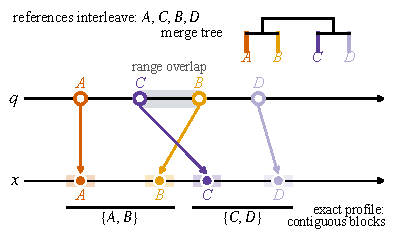
\includegraphics[width=\columnwidth]{figures/anchor_conflict_v23.pdf}
\caption{参考与拓扑的冲突。合并树要求块 $\{A,B\}$ 和 $\{C,D\}$，但参考位置的顺序是 $A,C,B,D$，因此每个精确剖面都必须把某些锚点移离其参考位置（箭头）。两棵子树参考范围的重叠（灰色）决定最小位移（定理~\ref{thm:order}）。位置为示意。}
\label{fig:projection_conflict}
\end{figure}
图~\ref{fig:projection_conflict} 给出冲突的最小实例。树把 $A$ 与 $B$、$C$ 与 $D$ 合并，因此精确剖面必须把 $\{A,B\}$ 和 $\{C,D\}$ 画成两个连续块。而参考位置的顺序是 $A,C,B,D$：$C$ 位于 $A$ 和 $B$ 之间，$B$ 位于 $C$ 和 $D$ 之间。两个块的任何一种顺序都不匹配，因此某些锚点必须离开参考位置，有限宽度还会带来额外的排布约束。它们必须移动多远只取决于树、参考位置、宽度和允许量，与绘制地图的算法无关。下一节计算这个量。

\section{保持树的位置代价}\label{sec:bounds}
现在我们依次回答引言中的三个问题：特征为点时精确的树迫使什么，有限宽度又增加什么，合并允许量能释放什么。每个下界只涉及 $T$、$q$、$W$ 和 $\eta$，因此无论权重或排序规则如何，它对式~\ref{eq:family} 的每个解都成立。补充材料给出完整证明。在一帧之内我们省略 $t$，记 $[v]^+=\max(v,0)$，并约定空集的最大值为零。

\subsection{精确拓扑}
考虑两棵兄弟子树 $X$ 和 $Y$，在等层级合并归为一个节点的约简树上，它们叶子的参考位置分别落在 $[m_X,M_X]$ 和 $[m_Y,M_Y]$。精确剖面必须把一个块完整地画在另一个之前。若 $X$ 在前，它的最高参考位置 $M_X$ 排在 $Y$ 的最低参考位置 $m_Y$ 之前，按 NROE 背后的论证，两个叶子之一至少移动 $[M_X-m_Y]^+/2$；另一种朝向的代价是 $[M_Y-m_X]^+/2$。即便是代价较小的朝向，也要付出剩余重叠的一半，而树中最坏的一对兄弟决定这个代价。
\begin{theorem}[精确拓扑位置下界]\label{thm:order}
每个满足 $\dtop=0$ 的剖面都有 $\nroe(\pi)\ge\nu^*(T,q)$，其中
\begin{equation}\label{eq:nu}
 \nu^*(T,q)=\frac{1}{2L}\max_v\max_{\substack{X,Y\in\mathrm{ch}(v)\\X\ne Y}}
 \bigl[\min(M_X-m_Y,\,M_Y-m_X)\bigr]^+ .
\end{equation}
把每个节点的子节点按其参考范围的中点排序，可在 $O(n\log n)$ 时间内达到 $\nu^*$。
\end{theorem}
\begin{proof}[证明概要]
中点排序为每对兄弟选择代价较小的朝向；而每对逆序的叶子都在其最低公共祖先处被两个兄弟块隔开，所以没有一个逆序的代价超过定义 $\nu^*$ 的那一对。
\end{proof}
定理~\ref{thm:order} 对点回答了前两个问题。精确的树的代价是最坏一对兄弟参考重叠的一半，取最大值的节点指出这份代价在树中出现的位置。在图~\ref{fig:projection_conflict} 中，$\{A,B\}$ 与 $\{C,D\}$ 的范围重叠 $q_B-q_C$，因此每个精确剖面的排序误差至少为 $(q_B-q_C)/2L$。

由于同一棵树的中点叶序达到 $\nu^*$，这个下界还把任何拓扑精确地图的排序误差分成两部分：树迫使的 $\nu^*$，以及地图的排序规则所选择、换用同一棵树的另一种叶序即可去掉的 $\nroe(\pi)-\nu^*$。NROE 不考虑宽度，因此这一划分同样适用于区间遵循不同规则的地图。

\subsection{有限宽度}
特征不是点。一个叶子块至少占据其宽度与间隔之和，所以即使两个兄弟块处于较好的朝向，也可能不得不把锚点推离参考位置，画布两端也带来同样的压力。对两个不相交的叶子集 $X$ 和 $Y$，令 $\omega(X,Y)$ 为把 $X$ 全部画在 $Y$ 之前（或相反）迫使其锚点承受的最小最坏位移，令 $E_\partial$ 为把所有区间放进画布两端之间所需的最小位移。两者都由排序后的参考端点和累积宽度得到。
\begin{theorem}[宽度感知位置下界]\label{thm:width}
令 $\mathcal{P}_0$ 包含两个兄弟节点的后代叶子集构成的每一对。每个拓扑精确的区间布局满足
\begin{equation}\label{eq:widthbound}
\begin{aligned}
 \|x-q\|_\infty\ge\tau(\pi)&\ge\mathcal{B}_w(T,q,W)\\
 &=\max\Bigl\{E_\partial,\max_{(X,Y)\in\mathcal{P}_0}\omega(X,Y)\Bigr\}.
\end{aligned}
\end{equation}
宽度和间隔为零时，$\mathcal{B}_w=L\,\nu^*(T,q)$。
\end{theorem}
\begin{proof}[证明概要]
一个块的首尾锚点必须在锚点松弛范围内包住其区间和间隔，这相对于它们的参考间距留下了缺口；精确的树为每对兄弟固定一种朝向，画布两端给出单侧代价。
\end{proof}
与 $\nu^*$ 不同，宽度下界 $\mathcal{B}_w$ 不一定能达到。当一张地图的区间代价超过它时，超出部分可能有一部分在下界本身。

\subsection{有界合并误差}
假设剖面可以把合并层级错报至多 $\eta$。这是否让它可以随意交错子树？不能。若叶子 $k$ 画在节点 $u$ 的两个后代 $i$ 与 $j$ 之间，$i$ 与 $j$ 之间的剖面经过 $k$，所以 $i$ 与 $k$ 的显示合并层级不能超过 $i$ 与 $j$ 的；两者误差都不超过 $\eta$，于是 $V_{ik}\le h(u)+2\eta$。因此，叶子 $k$ 只有在属于 $A_\eta(u)$ 的后代时才能进入 $u$ 的块，$A_\eta(u)$ 是层级与 $h(u)$ 相差不超过 $2\eta$ 的 $u$ 的最高祖先。令 $\mathcal{P}_\eta$ 包含这一规则保持分开的叶子集对：$\mathcal{D}(A_\eta(u))$ 之外的叶子 $k$ 构成的 $(\mathcal{D}(u),\{k\})$，以及满足 $\mathcal{D}(w)$ 与 $\mathcal{D}(A_\eta(u))$ 不相交、$\mathcal{D}(u)$ 与 $\mathcal{D}(A_\eta(w))$ 不相交的内部节点 $u,w$ 构成的 $(\mathcal{D}(u),\mathcal{D}(w))$，其中 $\mathcal{D}(\cdot)$ 表示后代叶子。
\begin{theorem}[有界拓扑位置下界]\label{thm:chain}
在每个满足 $\dtop\le\eta$ 的剖面中，$\mathcal{P}_\eta$ 的每一对都完整地以一种朝向绘制。因此
\begin{equation}\label{eq:chainbounds}
 \nroe(\pi)\ge C_\eta=\max_{(X,Y)\in\mathcal{P}_\eta}\frac{[\min(M_X-m_Y,M_Y-m_X)]^+}{2L},
\end{equation}
且 $\tau(\pi)$ 以定理~\ref{thm:width} 的表达式为下界，只需把 $\mathcal{P}_0$ 换成 $\mathcal{P}_\eta$。
\end{theorem}
定理~\ref{thm:chain} 回答了第三个问题。一旦 $2\eta$ 达到一棵子树自身合并层级与其父节点层级之间的差距，它就可以与兄弟交错。因此，在父节点之下不远处合并的子树之间的冲突很容易释放，而深处合并的冲突仍然代价高昂。把所有不超过 $2\eta$ 的父节点差距压平，可得到第二个有效下界；两者互不支配，我们报告较大者。反过来读，该定理也给另一端定价：排序误差低于 $C_\eta$ 的地图，例如排序误差为零的投影，其合并误差必然超过 $\eta$。

\section{AnchorMTM}\label{sec:method}
\begin{figure*}[t]
\centering
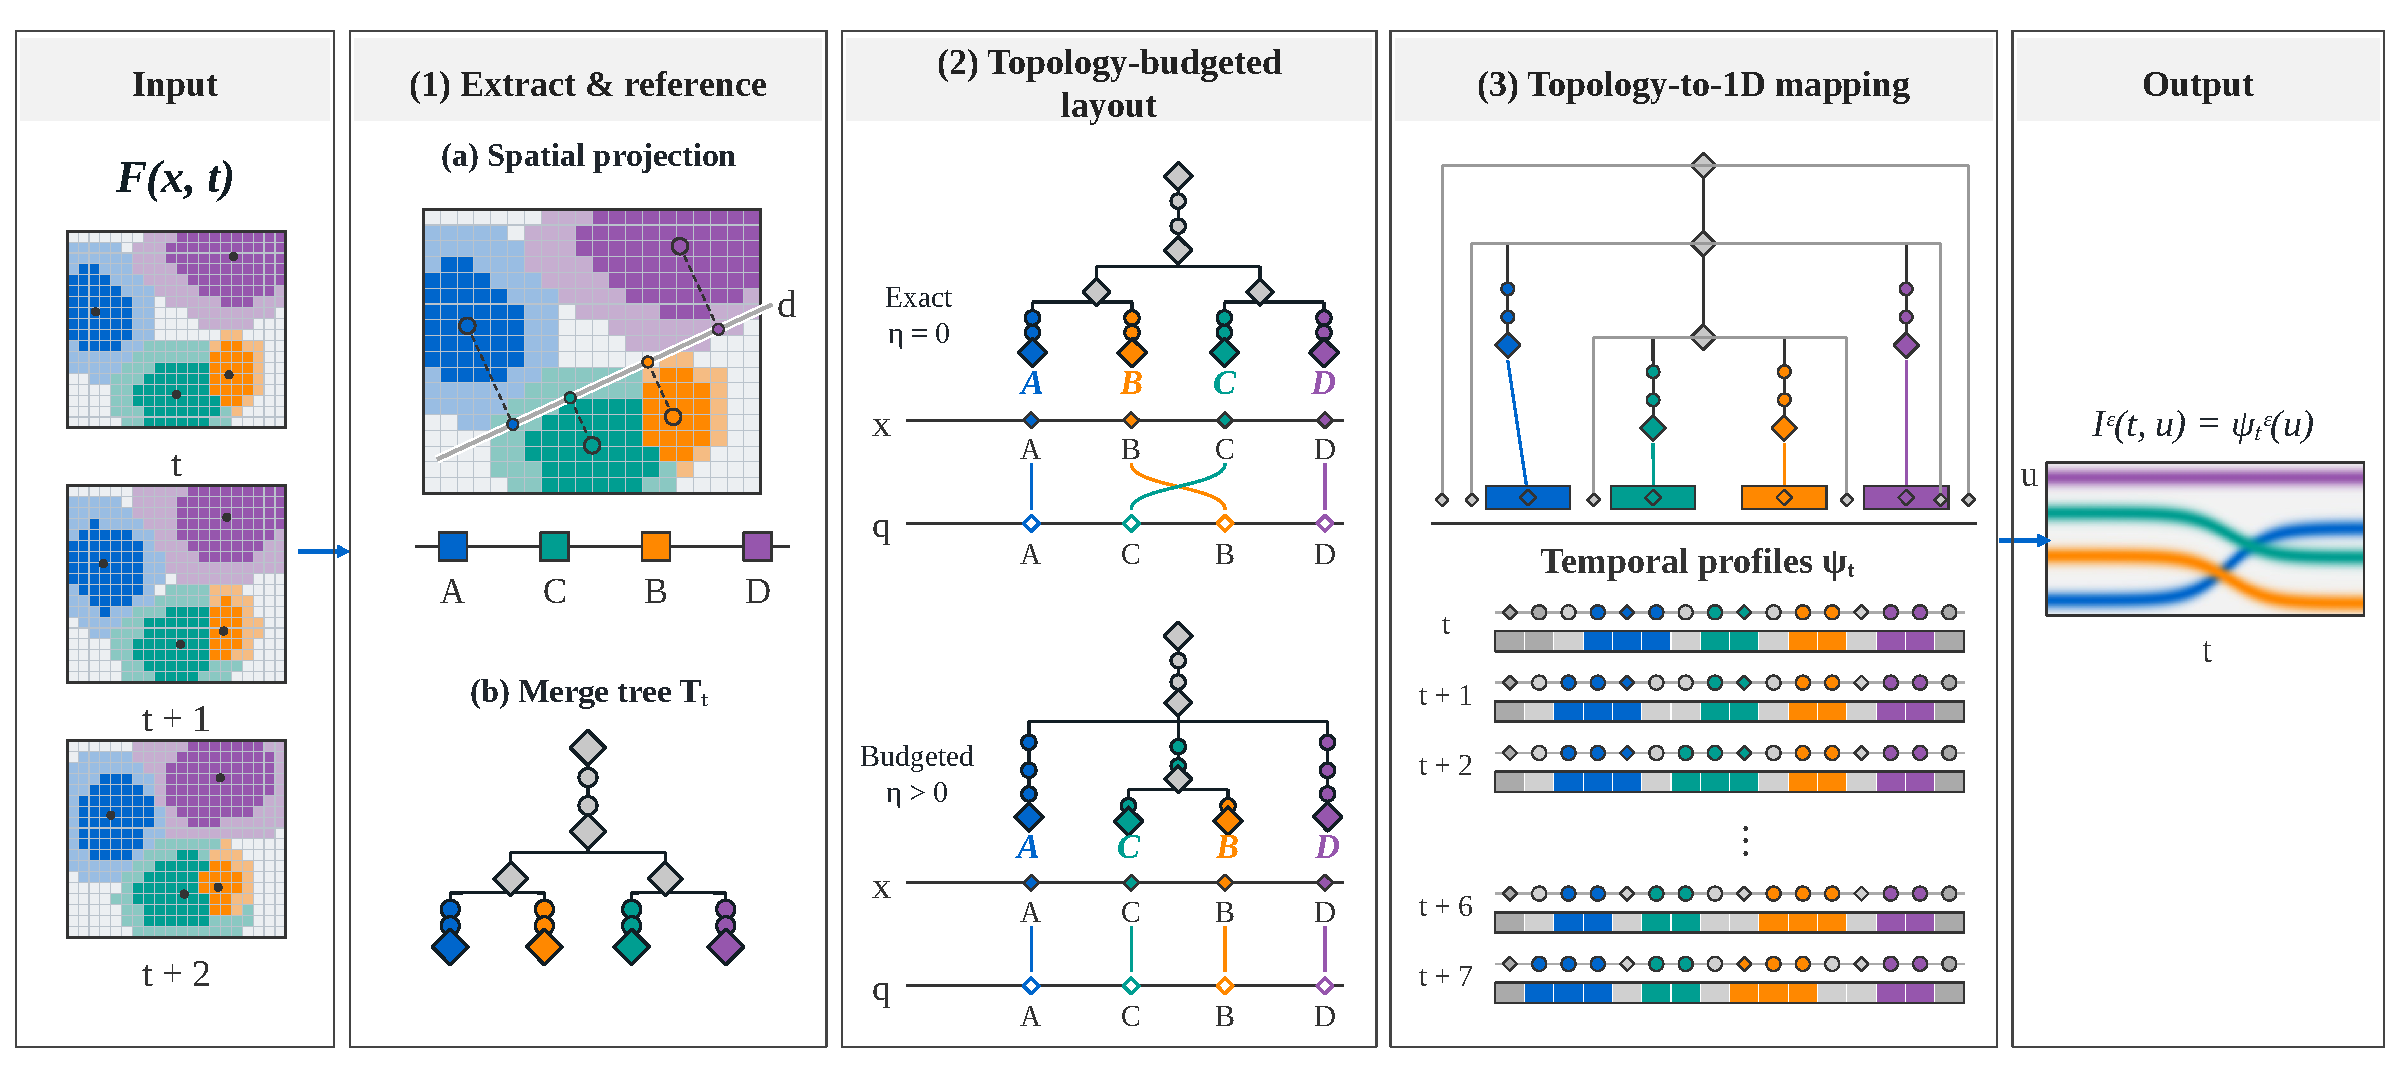
\includegraphics[width=\textwidth]{figures/anchor_framework.pdf}
\caption{AnchorMTM 的构建（$F(x,t)$：位置 $x$、时间 $t$ 处的场）。(1) 提取与参考：每帧的合并树、跨帧匹配的叶支撑，以及一个固定方向 $d$（式~\ref{eq:autodirection} 的 $a^*$），它给每个极值一个参考位置 $q$。(2) 拓扑预算布局：允许量 $\eta$ 所容许的叶序，然后在位移上限下放置锚点 $x$；$\eta=0$ 时叶序保持子树块、锚点离开参考位置，$\eta>0$ 时可以容许跟随参考位置的叶序。(3) 拓扑到一维的映射：区间和屏障填充每个剖面 $\psi_t$，剖面组成地图 $I^\varepsilon(t,u)=\psi^\varepsilon_t(u)$。图为示意。}
\label{fig:framework}
\end{figure*}
AnchorMTM 为序列的每一帧求解式~\ref{eq:family}，带参考项，允许量为 $\eta=(\varepsilon_0+\varepsilon)\Delta_F$。其中 $\Delta_F$ 是序列的标量范围，$\varepsilon_0=10^{-7}$ 是固定的数值容差，$\varepsilon\ge0$ 是预算，也是唯一的控制量。\emph{精确模式}（$\varepsilon=0$）在 $\varepsilon_0\Delta_F$ 之内的并列以外保持树，\emph{预算模式}（$\varepsilon>0$）以声明的合并误差换取位置。图~\ref{fig:framework} 给出三个阶段。第一阶段按上文计算树、匹配和参考，并给每个叶子宽度 $W_i=s\,m_i$，$s$ 是一个固定的尺度。式~\ref{eq:family} 把离散的叶序与连续的放置耦合在一起，第二阶段按下界所提示的方式把它们分开：先按下界所约束的量 $\tau$ 选择叶序，再放置锚点。第三阶段绘制并核验剖面。

\subsection{预算内的叶序}
一帧可以用哪些叶序？如果锚点之间的某种剖面能把合并误差保持在 $\eta$ 之内，这个叶序就是可容许的。这可以精确判定，因为对固定叶序，最优屏障有闭式解。
\begin{proposition}[最优屏障]\label{prop:barriers}
对固定叶序，令 $C_k=\min_{i\le k<j}V_{\pi(i)\pi(j)}$ 为跨越第 $k$ 个间隙的最低合并，$F_k$ 为其两侧极值中的较大者。可达到的最小合并误差为
\begin{equation}\label{eq:delta}
 \begin{split}
 \delta^*(\pi)=\max\Bigl\{&0,\;\max_k(F_k-C_k),\\
 &\tfrac12\max_{i<j}\bigl(V_{\pi(i)\pi(j)}-\max_{i\le k<j}C_k\bigr)\Bigr\},
 \end{split}
\end{equation}
由屏障 $b_k=C_k+\delta^*(\pi)$ 达到。
\end{proposition}
命题~\ref{prop:barriers} 把预算变成一个检验 $\delta^*(\pi)\le\eta$，并在叶序选定后确定屏障。正因如此，一个数就能控制整个构建。AnchorMTM 针对原始合并矩阵评估一个有限的候选叶序池：按中点排序的精确树（达到 $\nu^*$）；在阈值处和冲突合并处压平的树；以及宽度感知的块移动在细化其中最好者时经过的叶序。在可容许的候选中，它选出区间代价 $\tau$ 最小的一个，并以 NROE 打破平局。候选池是启发式的，所以所选叶序并未被证明在所有排列中最优；评估部分衡量它多频繁地达到下界。

\subsection{锚点放置}
叶序固定后，式~\ref{eq:family} 成为一个凸二次规划。AnchorMTM 使用权重 $(\lambda_R,\lambda_G,\lambda_M,\lambda_C)=(4,1,0.5,0.1)$ 和时间目标 $\hat x_i^t=x_{\mu_t(i)}^{t-1}+(q_i^t-q_{\mu_t(i)}^{t-1})$，它让锚点随其投影运动而移动，并使位移 $x-q$ 在时间上连续；没有匹配前驱的叶子没有时间项。该规划还满足上限 $\|x-q\|_\infty\le\tau(\pi)+\beta_0$，$\beta_0$ 是固定的松弛量。因为 $\tau$ 是可达的，这个上限可行，并把叶序的位置保证传给锚点：其他项塑造布局，却不能抵消叶序已取得的结果。

\subsection{剖面重建与核验}
剖面沿用早期合并树地图的叶弧采样和沿通往最低公共祖先路径的填充~\cite{Koepp:2023:TMTM,STMTM:2026}。极值留在其锚点上，随后每个间隙被削平或抬高到其屏障 $b_k$。所有帧共用方向、原点、长度和像素尺度，因此位置在不同时间和不同预算之间可比。栅格取整和严格极值间隙仍可能改变显示的合并层级，所以每个渲染帧都按原始合并矩阵核验，每一帧都记录所请求的预算、$\tau$、$\delta^*$ 和测得的误差。容量、输入和求解器的失败被报告出来，而不是通过重新缩放来修补。

\paragraph{计算。} AnchorMTM 不需要事先的布局：给定场和 $\varepsilon$，上述每一步都是确定的。在 Apple M2 Pro 上，下界每帧至多需要 5.5\,ms。在 Apple M4 上，对一个基准序列的完整运行需要 0.5--63\,s，其中排序和放置占 0.15--3.3\,s，其余是树的提取、匹配、栅格化和核验。744 帧的逐小时 PM$_{2.5}$ 序列在 $\varepsilon=5\%$ 时需要 231\,s。

\section{评估}\label{sec:experiments}
\definecolor{pubgray}{gray}{0.45}
\begin{table*}[t]
\centering
\caption{五组数据的比较。粗体与下划线标出每个数据集上本地测量的最优与次优值，并列者共享标记。曲线采用固定的默认朝向。}
\label{tab:quantitative-final}
\footnotesize
\setlength{\tabcolsep}{1.5pt}
\renewcommand{\arraystretch}{0.85}
\begin{tabular*}{\textwidth}{@{\extracolsep{\fill}}l*{12}{c}lccc@{}}
\toprule
\multirow{2}{*}{数据集} & \multicolumn{3}{c}{Hilbert} & \multicolumn{3}{c}{Morton} & \multicolumn{3}{c}{TMTM} & \multicolumn{3}{c}{ST-MTM} & \multicolumn{4}{c}{AnchorMTM（本文）} \\
\cmidrule(lr){2-4}\cmidrule(lr){5-7}\cmidrule(lr){8-10}\cmidrule(lr){11-13}\cmidrule(lr){14-17}
 & SNS$\downarrow$ & TW$\uparrow$ & NPE$\downarrow$ & SNS$\downarrow$ & TW$\uparrow$ & NPE$\downarrow$ & SNS$\downarrow$ & TW$\uparrow$ & NPE$\downarrow$ & SNS$\downarrow$ & TW$\uparrow$ & NPE$\downarrow$ & 模式 & SNS$\downarrow$ & TW$\uparrow$ & NPE$\downarrow$ \\
\midrule
\multirow{2}{*}{Gaussian} & \multirow{2}{*}{$0.1117$} & \multirow{2}{*}{$0.6719$} & \multirow{2}{*}{$0.7557$} & \multirow{2}{*}{$\underline{0.0393}$} & \multirow{2}{*}{$\underline{0.8333}$} & \multirow{2}{*}{$0.7359$} & \multirow{2}{*}{\textcolor{pubgray}{$0.2500^\dagger$}} & \multirow{2}{*}{\textcolor{pubgray}{$0.7700^\dagger$}} & \multirow{2}{*}{$\underline{0.1118}$} & \multirow{2}{*}{\textcolor{pubgray}{$0.0600^\dagger$}} & \multirow{2}{*}{\textcolor{pubgray}{$1.0000^\dagger$}} & \multirow{2}{*}{$0.1154$} & Exact & $\mathbf{0.0353}$ & $\mathbf{0.9323}$ & $\mathbf{0.0089}$ \\
 &  &  &  &  &  &  &  &  &  &  &  &  & Balanced & $\mathbf{0.0353}$ & $\mathbf{0.9323}$ & $\mathbf{0.0089}$ \\
\multirow{2}{*}{Ring} & \multirow{2}{*}{$\mathbf{0.1252}$} & \multirow{2}{*}{$\mathbf{0.9048}$} & \multirow{2}{*}{$0.5941$} & \multirow{2}{*}{$0.1489$} & \multirow{2}{*}{$0.7619$} & \multirow{2}{*}{$0.6033$} & \multirow{2}{*}{\textcolor{pubgray}{$0.2800^\dagger$}} & \multirow{2}{*}{\textcolor{pubgray}{$0.6800^\dagger$}} & \multirow{2}{*}{$0.1756$} & \multirow{2}{*}{\textcolor{pubgray}{$0.2100^\dagger$}} & \multirow{2}{*}{\textcolor{pubgray}{$0.8800^\dagger$}} & \multirow{2}{*}{$0.2463$} & Exact & $0.1485$ & $\underline{0.8571}$ & $\underline{0.0471}$ \\
 &  &  &  &  &  &  &  &  &  &  &  &  & Balanced & $\underline{0.1334}$ & $\underline{0.8571}$ & $\mathbf{0.0395}$ \\
\multirow{2}{*}{Wildfires} & \multirow{2}{*}{$0.1883$} & \multirow{2}{*}{$0.8303$} & \multirow{2}{*}{$0.3641$} & \multirow{2}{*}{$0.1304$} & \multirow{2}{*}{$0.8758$} & \multirow{2}{*}{$0.1560$} & \multirow{2}{*}{\textcolor{pubgray}{$0.4400^\dagger$}} & \multirow{2}{*}{\textcolor{pubgray}{$0.8800^\dagger$}} & \multirow{2}{*}{$0.2280$} & \multirow{2}{*}{\textcolor{pubgray}{$0.2400^\dagger$}} & \multirow{2}{*}{\textcolor{pubgray}{$0.9100^\dagger$}} & \multirow{2}{*}{$0.3180$} & Exact & $\mathbf{0.0426}$ & $\mathbf{0.9136}$ & $\underline{0.0131}$ \\
 &  &  &  &  &  &  &  &  &  &  &  &  & Balanced & $\underline{0.0447}$ & $\underline{0.8989}$ & $\mathbf{0.0116}$ \\
\multirow{2}{*}{Storms} & \multirow{2}{*}{$0.1290$} & \multirow{2}{*}{$0.7403$} & \multirow{2}{*}{$0.3705$} & \multirow{2}{*}{$0.1180$} & \multirow{2}{*}{$0.7251$} & \multirow{2}{*}{$0.3468$} & \multirow{2}{*}{\textcolor{pubgray}{$0.3400^\dagger$}} & \multirow{2}{*}{\textcolor{pubgray}{$0.7100^\dagger$}} & \multirow{2}{*}{$0.5753$} & \multirow{2}{*}{\textcolor{pubgray}{$0.2100^\dagger$}} & \multirow{2}{*}{\textcolor{pubgray}{$0.9400^\dagger$}} & \multirow{2}{*}{$0.4579$} & Exact & $\underline{0.0790}$ & $\underline{0.8463}$ & $\underline{0.0399}$ \\
 &  &  &  &  &  &  &  &  &  &  &  &  & Balanced & $\mathbf{0.0743}$ & $\mathbf{0.8766}$ & $\mathbf{0.0140}$ \\
\multirow{2}{*}{PM$_{2.5}$} & \multirow{2}{*}{$0.2386$} & \multirow{2}{*}{$\mathbf{0.8887}$} & \multirow{2}{*}{$0.8090$} & \multirow{2}{*}{$\underline{0.1760}$} & \multirow{2}{*}{$\underline{0.8277}$} & \multirow{2}{*}{$0.8823$} & \multirow{2}{*}{$0.3018$} & \multirow{2}{*}{$0.7781$} & \multirow{2}{*}{$0.5241$} & \multirow{2}{*}{$0.1897$} & \multirow{2}{*}{$0.8224$} & \multirow{2}{*}{$0.5577$} & Exact & $0.1964$ & $0.7884$ & $\underline{0.1390}$ \\
 &  &  &  &  &  &  &  &  &  &  &  &  & 5\% & $\mathbf{0.1636}$ & $0.7657$ & $\mathbf{0.0468}$ \\
\bottomrule
\end{tabular*}
\vspace{2pt}
\begin{minipage}{\textwidth}\footnotesize $^\dagger$灰色：ST-MTM 论文表~1 中在作者输入上发表的 TMTM/ST-MTM 时间模式 SNS/TW，仅供参照，不参与标记；其余各项（含全部 PM$_{2.5}$ 数值）均为相同输入上的本地测量。作者输入与覆盖范围未经确认。本地 TW 的覆盖帧数（Gaussian/Ring/Wildfires/Storms/PM$_{2.5}$）为 64/64、1/40、4/32、11/744、744/744，不符合条件的帧略去。已发表的 TW 精确到两位小数。模式仅适用于 AnchorMTM；PM$_{2.5}$ 采用固定的 5\% 预算，并非选定的 Balanced 预算。\end{minipage}
\end{table*}

\begin{figure}[t]
\centering
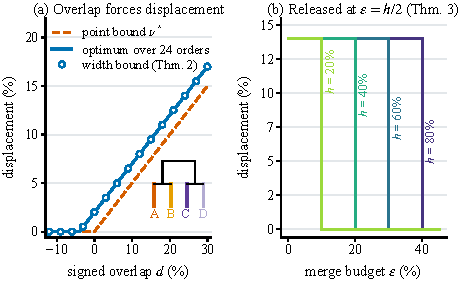
\includegraphics[width=\columnwidth]{figures/anchor_controlled_bounds.pdf}
\caption{图~\ref{fig:projection_conflict} 构型下的受控四叶树（插图）。(a) 兄弟范围的重叠 $d$ 增大会迫使位移；定理~\ref{thm:width} 的宽度下界（圆点）等于全部 24 种叶序中的最优值。(b) 在 $d=24\%$ 时，当合并预算达到父节点差距 $h$ 的一半时，14\% 的位移恰好消失，四种差距都如此，正如定理~\ref{thm:chain} 所预言。百分比相对于单位画布或单位标量范围。}
\label{fig:controlled}
\end{figure}
\begin{figure*}[t]
\centering
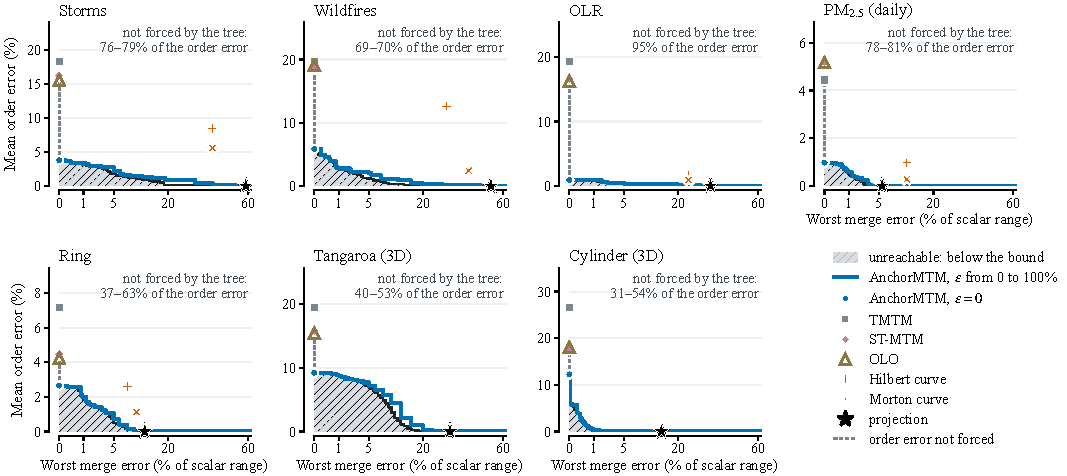
\includegraphics[width=\textwidth]{figures/plane_compact.pdf}
\caption{七个下界组序列的位置--拓扑平面。每张地图是一个点，横坐标为其各帧中的最坏合并误差（平方根刻度），纵坐标为其平均排序误差。没有地图能进入下界之下的阴影区域（定理~\ref{thm:chain} 与压平下界；零合并误差处为定理~\ref{thm:order}）。TMTM、ST-MTM 和 OLO 保持树，位于零合并误差处、远高于下界；虚线段是它们未被树迫使的排序误差，标注给出其占比。空间填充曲线和投影跟随空间、破坏树。AnchorMTM（蓝线，$\varepsilon$ 从 0 到 100\%；圆点，$\varepsilon=0$）沿该区域的边缘延伸。TMTM、ST-MTM 和 OLO 取与参考更一致的镜像。}
\label{fig:plane}
\end{figure*}
我们检验四个论断，每个对应一小节：下界是紧的；已有地图的大部分位置误差并非由树迫使；在相同的拓扑保证下，AnchorMTM 把特征画在它们所在的位置；预算在冲突较浅之处换来位置。

\subsection{数据与度量}\label{sec:data}
\begin{table}[t]
\centering
\caption{两组序列。下界组复用早期基准保存的树和一组默认配置；布局组重建 ST-MTM 基准，并加入一个逐小时 PM$_{2.5}$ 序列和 TMTM 的体数据。}
\label{tab:data}
\footnotesize
\setlength{\tabcolsep}{2pt}
\renewcommand{\arraystretch}{0.95}
\begin{tabular*}{\columnwidth}{@{\extracolsep{\fill}}lllrl@{}}
\toprule
组 & 序列 & 场 & 帧数 & 小节 \\
\midrule
下界组 & Storms~\cite{Hersbach:2020:ERA5} & ERA5 海平面气压（12 小时） & 118 & \ref{sec:bounds-eval}, \ref{sec:eval-forced} \\
 & Wildfires~\cite{Franke:2021:1DP} & 火辐射功率，逐日 & 30 & \\
 & OLR~\cite{NOAA:OLR} & 向外长波辐射 & 60 & \\
 & PM$_{2.5}$~\cite{Dong:2026:PM25} & PM$_{2.5}$ 浓度，逐日 & 366 & \\
 & Ring & 合成圆环 & 40 & \\
 & Tangaroa~\cite{Popinet:2004:Tangaroa} & 速度大小（三维） & 201 & \\
 & Cylinder~\cite{Camarri:2005:Cylinder} & $Q$ 判据（三维） & 102 & \\
\midrule
布局组 & Gaussian & 三个移动的峰 & 64 & \ref{sec:eval-placement}, \ref{sec:eval-budget} \\
 & Ring & 合成圆环 & 40 & \\
 & Wildfires & 火辐射功率（32 个时段） & 32 & \\
 & Storms & ERA5 气压距平（1 小时） & 744 & \\
 & PM$_{2.5}$~\cite{Kong:2021:CAQRA} & PM$_{2.5}$ 浓度，逐小时 & 744 & \\
 & Tangaroa & 速度大小（三维） & 201 & \\
 & Cylinder & $Q$ 判据（三维） & 102 & \\
\bottomrule
\end{tabular*}
\end{table}

\paragraph{数据。} 表~\ref{tab:data} 列出两组序列，每组各有其用途。\emph{下界组}由七个序列组成，它们的树、匹配和参考由同一个早期流程保存。由于这些树是固定的，我们用它们计算下界、枚举小帧的全部叶序，并逐帧度量每张对比地图。\emph{布局组}从场重新计算树，比较完整的地图。它重建 ST-MTM 基准的四个平面输入~\cite{STMTM:2026}，使 AnchorMTM 在最接近的已有工作的数据上接受比较，并加入华北地区的逐小时 PM$_{2.5}$ 序列~\cite{Kong:2021:CAQRA}和 TMTM 的两组体数据~\cite{Koepp:2023:TMTM,Weinkauf:SquareCylinder}。Ring、Storms、Wildfires 和体数据在两组中都出现，但预处理不同；逐日和逐小时的 PM$_{2.5}$ 序列是不同的数据。ST-MTM 基准的作者处理数组无法获得，因此布局组是公开说明的重建，而非相同输入的复现；补充材料给出每个序列的预处理。

\paragraph{度量。} NMLE 是渲染剖面的合并误差 $\dtop$ 除以标量范围，NROE 是式~\ref{eq:nroe} 的排序误差。NPE 是一帧的最坏位移除以长度 $L$ 后在各帧上的平均；它是读轴的人所感受到的误差。为体现 ST-MTM 的目标，我们还报告锚点距离相对支撑质心距离的尺度归一化应力（SNS）~\cite{Smelser:2025:Scale,STMTM:2026}和可信度（TW）~\cite{Venna:2001:NP}。基线是我们对已发表方法的实现，使用相同的树、标识和参考。在四个基准输入上，TMTM 和 ST-MTM 的 SNS 和 TW 引自 ST-MTM 论文（表~\ref{tab:quantitative-final} 中灰色），不与本地数值排名。TMTM 和 ST-MTM 都不固定其轴的方向，因此每个基线在每个序列上翻转一次，使之与参考一致。

\paragraph{模式。} Exact 即精确模式。Balanced 是预算模式，其预算在每个序列前四分之一的时间段上从 1--10\% 中选定一次后冻结：Gaussian、Ring、Wildfires 和 Storms 分别为 1、1、5 和 10\%。逐小时 PM$_{2.5}$ 使用固定的 5\% 预算。表~\ref{tab:volume-comparison} 中的体数据使用存储的配置和 $+x$ 参考；图~\ref{fig:volume-gallery} 和图~\ref{fig:budget-distribution} 使用下界组的默认配置。补充材料列出全部设置和预算选择。

\subsection{下界是紧的}\label{sec:bounds-eval}
\emph{受控树。} 我们先在已知最优值的情形下检验下界。两对兄弟 $\{A,B\}$ 和 $\{C,D\}$ 在 $0.4$ 处合并，根在 $1$，叶子数值为 $0$，单位画布上的参考位置为 $(0.2,0.5,0.5-d,0.8-d)$；$0<d<0.3$ 时这正是图~\ref{fig:projection_conflict} 的顺序 $A,C,B,D$。在 $d$ 从 $-0.12$ 到 $0.30$ 的 43 个重叠和四种宽度下，我们把下界与全部 24 种叶序比较，每种叶序由一个独立的极小极大线性规划放置。仅拓扑就恰好迫使 $\nu^*=\max(0,d)/2$。当宽度为 $0.06$、间隔为 $0.01$、$\rho=0.5$ 时，宽度下界、我们的搜索与穷举最优值在 $\tau=\max(0,(d+0.04)/2)$ 处重合（图~\ref{fig:controlled}a）：在 $d=0.24$ 时，点为 12\%，区间为 14\%。合并预算恰好在定理~\ref{thm:chain} 容许交错之处消除冲突，对全部四个父节点差距 $h$ 都在 $2\varepsilon=h$ 处（图~\ref{fig:controlled}b）。

\emph{真实树。} 同样的吻合在真实数据上也成立。在精确模式下，所选叶序的区间代价 $\tau$ 在下界组 614 个平面帧中的 606 个上等于 $\mathcal{B}_w$，因此在这些帧上没有拓扑精确的叶序有更小的最坏位移；在 $\varepsilon=10\%$ 时，有界拓扑下界在 596 帧上达到。在 Storms、OLR、逐日 PM$_{2.5}$ 和 Ring 上，每帧至多八个叶子，枚举全部叶序证实 AnchorMTM 在每个测试预算下都达到最小排序误差，只有 Storms 的一帧在 $\varepsilon=31.6\%$ 时例外（1.9 个百分点）。体数据更难：宽度下界在 102 个 Cylinder 帧中的 81 个、201 个 Tangaroa 帧中的 27 个上达到，其余差距可能在下界中，也可能在启发式搜索中。

\subsection{已有地图付出的超过树的要求}\label{sec:eval-forced}
定理~\ref{thm:order} 不需要布局，因此它能度量每张保持树的地图。在七个下界组序列上，TMTM 排序误差的 53--95\% 和 ST-MTM 的 31--95\% 高于 $\nu^*$；换用同一棵树的另一种叶序即可去掉这一部分。最优叶序（OLO）只在树内让相似叶子相邻，表现相同（32--95\%）。因此，超出的部分来自在没有空间参考的情况下选择叶序，而不是某一种特定方法。图~\ref{fig:plane} 把每张地图放进由两种误差张成的平面。保持树的地图位于零合并误差处、远高于下界。投影只有在合并误差达到 5.6--59\% 时才达到零排序误差，空间填充曲线也破坏树（8--40\%）。AnchorMTM 沿不可达区域的边缘延伸，这条边缘显示预算能释放什么。在冲突子树于父节点之下不远处合并的地方，1\% 的预算把 Wildfires 上被迫使的排序误差减半（5.80\% 到 2.77\%），几乎消除 Cylinder 上的（12.24\% 到 0.23\%）；Tangaroa 的深层冲突使其在 $\varepsilon=5\%$ 之前一直高于 7\%。被迫使的误差还取决于方向，并能在画图之前算出：在 400 个方向上，它在 Tangaroa 上为 4.70--10.14\%，在 Cylinder 上为 5.49--28.15\%。

\subsection{特征位于它们所在的位置}\label{sec:eval-placement}
\begin{table}[t]
\centering
\caption{固定 $x$ 参考方向下的体数据比较。粗体与下划线标出每个数据集上的最优与次优值，并列者共享标记。}
\label{tab:volume-comparison}
\footnotesize
\setlength{\tabcolsep}{1.2pt}
\renewcommand{\arraystretch}{0.9}
\begin{tabular*}{\columnwidth}{@{\extracolsep{\fill}}lccc lccc@{}}
\toprule
\multirow{2}{*}{数据集} & \multicolumn{3}{c}{TMTM} & \multicolumn{4}{c}{AnchorMTM（本文）} \\
\cmidrule(lr){2-4}\cmidrule(lr){5-8}
 & SNS$\downarrow$ & TW$\uparrow$ & NPE$\downarrow$ & 模式 & SNS$\downarrow$ & TW$\uparrow$ & NPE$\downarrow$ \\
\midrule
\multirow{2}{*}{Cylinder} & \multirow{2}{*}{$0.2956$} & \multirow{2}{*}{$\underline{0.8017}$} & \multirow{2}{*}{$0.4769$} & Exact & $\underline{0.1226}$ & $0.8010$ & $\underline{0.1773}$ \\
 &  &  &  & Balanced & $\mathbf{0.0329}$ & $\mathbf{0.9117}$ & $\mathbf{0.0458}$ \\
\multirow{2}{*}{Tangaroa} & \multirow{2}{*}{$0.5255$} & \multirow{2}{*}{$0.6701$} & \multirow{2}{*}{$0.3866$} & Exact & $\underline{0.1204}$ & $\underline{0.8213}$ & $\underline{0.1285}$ \\
 &  &  &  & Balanced & $\mathbf{0.1124}$ & $\mathbf{0.8408}$ & $\mathbf{0.0653}$ \\
\bottomrule
\end{tabular*}
\vspace{2pt}
\begin{minipage}{\columnwidth}\footnotesize 全部为本地测量，包括改编后的 TMTM。TW 取 $k=1$，覆盖 102/102 和 201/201 帧。模式仅适用于 AnchorMTM。各配置为冻结的探索性结果，并非盲测；设置见补充材料。\end{minipage}
\end{table}

\begin{figure*}[t]
\centering
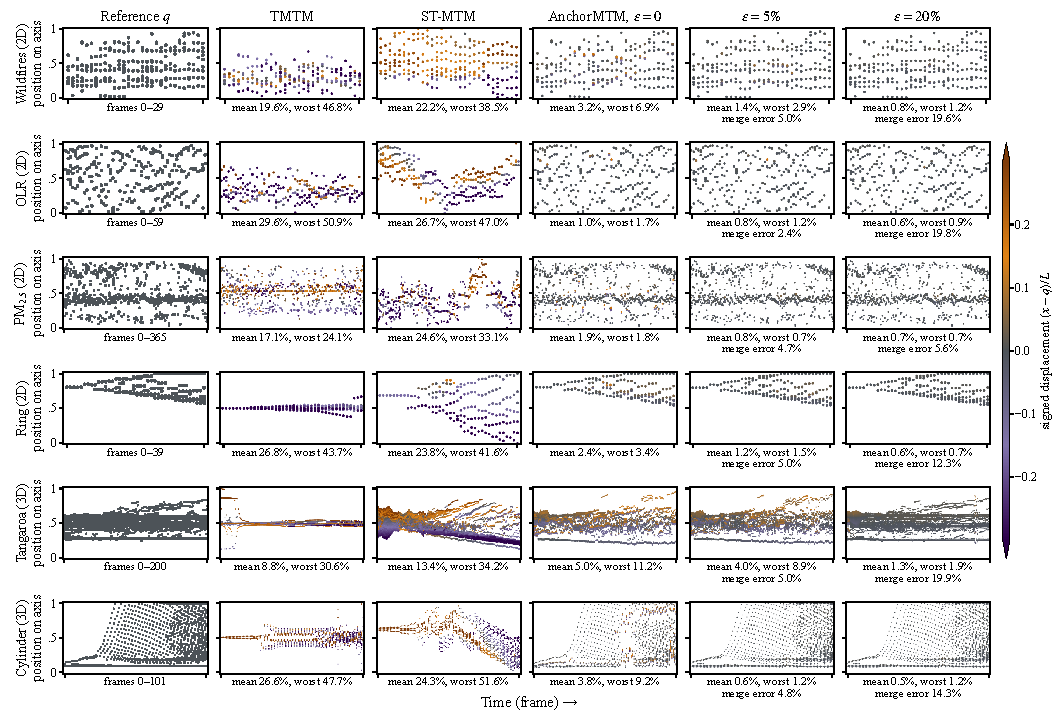
\includegraphics[width=\textwidth]{figures/volume_gallery.pdf}
\caption{各方法把两组体数据的特征画在哪里。每个点是一帧中的一个特征，位于其在轴上的位置（画布的比例），颜色表示它相对参考的有符号位移；灰点位于参考位置上。第一列给出参考位置，即把地图读作位置时应当看到的内容。所有方法使用相同的树和特征，TMTM 和 ST-MTM 取与参考更一致的镜像。AnchorMTM 使用默认配置，参考取匹配运动方向（Tangaroa）或顺流 $x$ 轴（Cylinder）。每个面板下方：各帧上的平均位移和平均最坏位移，以及正预算下实际达到的合并误差。}
\label{fig:volume-gallery}
\end{figure*}
\emph{平面输入。} 在精确保持树的条件下，Exact 在表~\ref{tab:quantitative-final} 的全部五个平面输入上把 NPE 相对 TMTM 和 ST-MTM 降低 73--96\%（PM$_{2.5}$ 上为 73.5 和 75.1\%），也低于破坏树的 Hilbert 和 Morton 曲线。Balanced 的预算至多 10\%，它相对 Exact 进一步把 NPE 在 Ring 上降低 16.2\%、在 Wildfires 上降低 11.6\%、在 Storms 上降低 64.9\%；在 Gaussian 上地图不变，在 PM$_{2.5}$ 上固定的 5\% 预算把 NPE 降低 66.3\%。这些结果表明的是与所选参考的对齐，而不是质量的全面提升。ST-MTM 在全部四个基准输入上报告了更高的 TW。在所有分数都在本地测得的 PM$_{2.5}$ 上，ST-MTM 的 SNS 也低于、TW 也高于 Exact（0.1897 和 0.8224 对 0.1964 和 0.7884）。与曲线相比，Balanced 在 Gaussian、Wildfires 和 Storms 上改进了 SNS 和 TW；Hilbert 在 Ring 上更好（SNS 0.1252、TW 0.9048 对 0.1334、0.8571，TW 只来自一个合格帧），两条曲线在 PM$_{2.5}$ 上的 TW 都高于 5\% 地图。

\emph{一个风暴。} 图~\ref{fig:storms_overview} 展示这些平均值对单个特征意味着什么。风暴从大西洋移向斯堪的纳维亚时，它的参考位置从轴的 0.08 升到 0.86。TMTM 按时间重叠对齐子树，ST-MTM 按相对距离放置它们，所以两者都把风暴保持在中部附近，它的条带既不传达位置也不传达运动方向。在精确的树下，AnchorMTM 把风暴画得离参考位置平均为轴长的 1.5\%，10\% 的预算把它降到 1.0\%。这些地图使用 Storms 场的逐小时档案；基线在相同的 744 个场和树上运行。

\emph{运动的读取。} 空间轴还应显示两个特征是在靠近还是在分离。在下界组含此类事件的四个平面序列上（Storms、Wildfires、OLR 和 Ring；56--124 个事件，事件指两个被追踪特征之间的距离在两帧内变化超过区域对角线的 2\%），精确模式的 AnchorMTM 把 5--35\% 的事件显示为方向错误或没有显示，TMTM 为 39--65\%，ST-MTM 为 21--41\%，且两个基线在任何序列上都没有错读更少的事件。由于我们放置中的运动项奖励这一行为，这一结果说明的是该轴支持运动的读取，而不是提供独立证据。

\emph{体数据。} 在表~\ref{tab:volume-comparison} 的存储配置和 $+x$ 参考下，Exact 在零合并误差时把 NPE 在 Cylinder 上从 0.477 降到 0.177，在 Tangaroa 上从 0.387 降到 0.129，Balanced 在全部三项度量上都优于 TMTM；Tangaroa 的 33.33\% 预算和以几何为主的权重限制了归因。图~\ref{fig:volume-gallery} 在默认配置下展示这些数字背后的位置。TMTM 和 ST-MTM 把 Cylinder 的涡集中在轴的中部附近（平均最坏位移 47.7\% 和 51.6\%），而 Exact 已经再现了参考位置所呈现的脱落模式（9.2\%），5\% 的预算几乎去掉了其余部分（1.2\%）。Tangaroa 的冲突位于树的深处：Exact 把 30.6\%（TMTM）和 34.2\%（ST-MTM）降到 11.2\%，参考位置的模式只在 $\varepsilon=20\%$ 附近才出现（1.9\%）。

\emph{预算得到遵守。} Exact 在每个输入上测得的合并误差都为零，Balanced 至多达到 0、0.982、4.421 和 9.985\%，均在其预算之内。所有运行都通过连续和栅格核验，没有锚点塌缩；Ring 在 26 个 Exact 帧和 21 个 Balanced 帧中需要经过核验的联合整数取整。在体数据的扫描中，全部 1,515 个渲染帧都按其叶子的合并矩阵重新核验，没有违规。核验覆盖极值，而非增广树的每个内部标签。

\subsection{预算在哪里起作用}\label{sec:eval-budget}
\begin{figure*}[t]
\centering
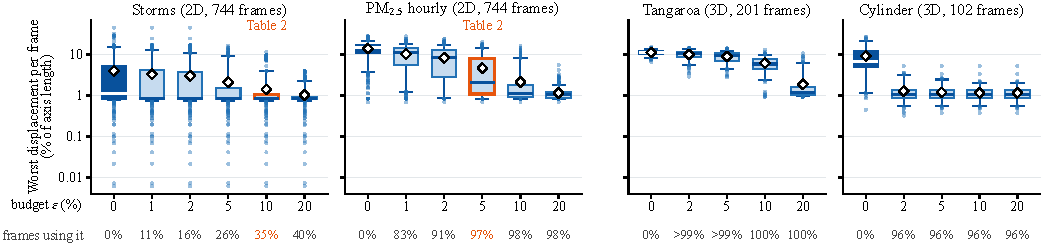
\includegraphics[width=\textwidth]{figures/budget_per_frame.pdf}
\caption{完整序列上 AnchorMTM 每帧最坏位移随合并预算 $\varepsilon$ 的变化（对数刻度）：两个平面输入使用表~\ref{tab:quantitative-final} 的配置，两组体数据使用默认配置。箱体：四分位数；须：第 5--95 百分位；点：须之外的所有帧；菱形：均值，即表中的 NPE；深色：Exact；橙色：表~\ref{tab:quantitative-final} 的预算。底行给出实际合并误差为正的帧所占比例；没有帧超出其预算。}
\label{fig:budget-distribution}
\end{figure*}
预算限制的是合并误差而非位移，所以它对地图的作用取决于有多少帧含有它能释放的冲突（图~\ref{fig:budget-distribution}）。在 Storms 上，$\varepsilon=10\%$ 时 35\% 的帧用到允许量，集中在几段连续的帧中。因此预算缩短了上尾：每帧位移的中位数只从 1.10\% 变到 0.84\%，而第 90 百分位从 10.7\% 降到 2.5\%，最坏帧从 44.8\% 降到 11.5\%。在逐小时 PM$_{2.5}$ 上，97\% 的帧用到 5\% 的预算，整个分布下移：中位数从 14.5\% 降到 2.1\%。体数据表现相同。在 $\varepsilon=2\%$ 时，201 个 Tangaroa 帧中的 200 个和 102 个 Cylinder 帧中的 98 个用到预算；Cylinder 的中位数在 2\% 时就从 6.8\% 降到 1.0\%，Tangaroa 的中位数在 20\% 时从 11.3\% 降到 1.2\%。在 Wildfires 上，同样的 32 帧中的 7 帧在每个预算下用到允许量；在 Ring 上，中位数从 3.9\% 降到 1.0\%，而最后一帧在预算达到 63\% 之前一直停在 10.0\%。在 Gaussian 上，预算不改变任何一帧。补充材料给出所有序列的这些分布，以及一个从地图读出的逐小时 PM$_{2.5}$ 污染过程。

\section{讨论与局限}
\paragraph{下界的用途。} 下界把任何合并树地图的位置误差分成树迫使的部分和布局选择的部分。高于 $\nu^*$ 的排序误差总能在不改变树的情况下去掉，因为中点排序达到 $\nu^*$。宽度感知下界和有界拓扑下界不一定能达到，因此超出它们的部分可能有一部分在下界本身。由于下界只需要树、参考位置和宽度，分析人员可以在画图之前算出它们，用来比较候选方向或判断一份预算是否值得花，并且任何这类新布局都可以拿来与它们比较。

\paragraph{位置与邻域。} 固定的空间参考和面向几何的嵌入回答不同的问题。AnchorMTM 支持沿所选方向读取位置和运动，而 ST-MTM 更高的 TW 说明了保持局部邻域的价值；两种性质互不保证。我们的结果支持这一面向任务的论断，而不是空间或时间保真度上的全面优势。一条轴也只承载一个坐标。要读取二维位置，需要沿另一方向再画一张地图，并有其自身的下界。

\paragraph{局限。} 作者处理的场及其小样本 TW 协议无法完全获得，因此已发表的 SNS 和 TW 不能支持相同输入的显著性检验，两组数据的预处理也不同。默认参考和轨迹由整个序列离线计算，因此在线使用需要事先选定方向；支撑重叠只是对应关系的代理，而非物理身份。叶序搜索是启发式的，连续的证书也不能消除栅格取整；因此我们核验渲染出的合并矩阵，但并非增广树的每个内部标签。我们尚未测量感知上的可读性或人对运动判断的准确性；这些需要用户研究。

\section{结论}
给合并树地图一条空间轴有一份无法避免的位置代价，而这份代价可以在画图之前由数据算出。AnchorMTM 只比这份代价多付出少许。在精确保持树的条件下，它的叶序在 614 个平面帧中的 606 个上达到下界，并在五个平面输入上把 TMTM 和 ST-MTM 的平均最坏位移降低 73--96\%；它们的排序误差大部分并非由树迫使。一个在每个渲染帧上都经过核验的合并误差预算，在冲突较浅之处换来更多的位置，而下界事先指出它会在哪里起作用。
\FloatBarrier
\begingroup
\interlinepenalty=10000
\bibliographystyle{abbrv-doi-narrow}
\bibliography{refs}
\endgroup
\end{document}
